\documentclass[letterpaper,12pt]{article}
\usepackage{subfiles,amsmath,amssymb,float,epstopdf}
\numberwithin{equation}{subsection}
\bibliographystyle{plain}
\usepackage[margin=1.0in]{geometry}
\usepackage[hypcap]{caption}
\usepackage{subcaption}
\usepackage{hyperref}
\usepackage{indentfirst}
\usepackage{graphicx}
\usepackage{setspace}
\doublespacing
\graphicspath{ {./img/} }

\begin{document}

\title{\textbf{Advanced Monte Carlo: Ising Model}}
\author{Jacob Calcutt,\\
	Gregorio Ponti,\\
	Physics 480, \\
	Computational Physics,\\
	Spring 2015\\
	Michigan State University}
\maketitle

\newpage
\tableofcontents

\newpage
\section{Introduction}
I STICK MA DICK IN THE OWL
\subsection{Ising Model}
\begin{figure}[H]
        \centering
        \caption{Sample of the vis we want \label{fig:blah}}
    %    \begin{subfigure}[b]{\textwidth}
                \centering
                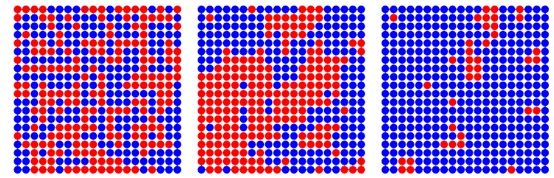
\includegraphics[width=0.75\textwidth]{sample_lattice.png}
    %    \end{subfigure}
\end{figure}

\newpage

\subsection{Initialization}

\subsection{Wolff Algorithm}
\subsection{Calculations}
\subsubsection{Magnetization}
\subsubsection{Magnetic Susceptibility}
\begin{equation}
\chi = \dfrac{d(Magnetization)}{dT}
\end{equation}
\subsubsection{Critical Temperature}
\subsubsection{Internal Energy}
\begin{equation}
E = - J \cdot \Sigma_{<i><j>} S_i S_j
\end{equation}
\subsubsection{Heat Capacity}
\begin{equation}
C_V = \dfrac{dE}{dT}
\end{equation}
\subsubsection{Critical Exponents}

\newpage
\section{Results}
\subsection{Magnetization}
%\begin{figure}[H]
%        \centering
%        \caption{Magnetization vs Temperature \label{fig:magvsT}}
%    %    \begin{subfigure}[b]{\textwidth}
%                \centering
%                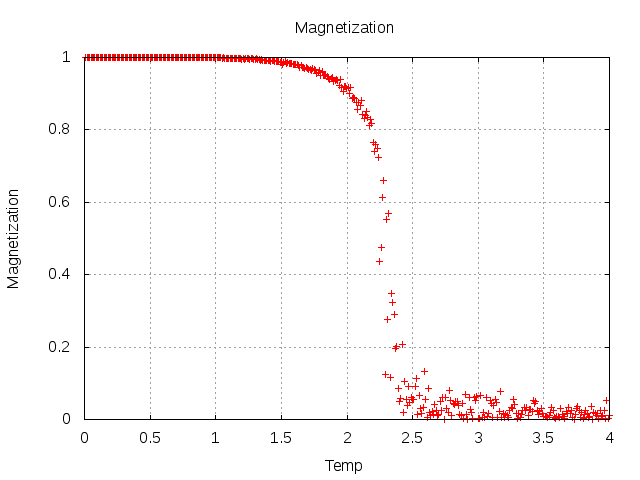
\includegraphics[width=0.75\textwidth]{MagVsT.png}
%    %    \end{subfigure}
%\end{figure}
\subsection{Magnetic Susceptibility}
%\begin{figure}[H]
%        \centering
%        \caption{Magnetic Susceptibility vs Temperature \label{fig:chivsT}}
%    %    \begin{subfigure}[b]{\textwidth}
%                \centering
%                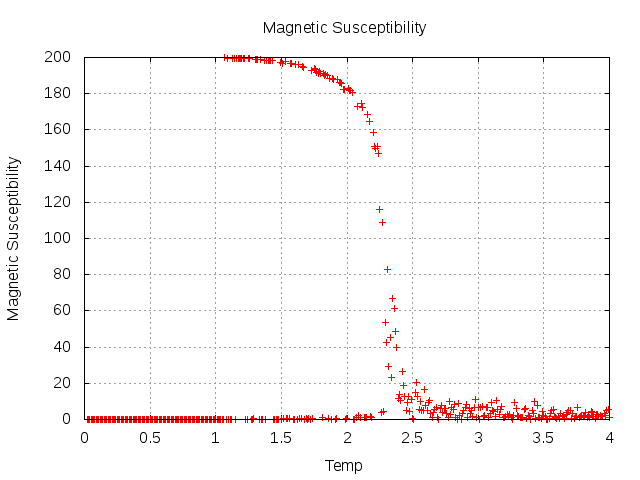
\includegraphics[width=0.75\textwidth]{chiVsT.png}
%    %    \end{subfigure}
%\end{figure}
\subsection{Critical Temperature}
\subsection{Internal Energy}
%\begin{figure}[H]
%        \centering
%        \caption{Internal Energy vs Temperature \label{fig:EvsT}}
%    %    \begin{subfigure}[b]{\textwidth}
%                \centering
%                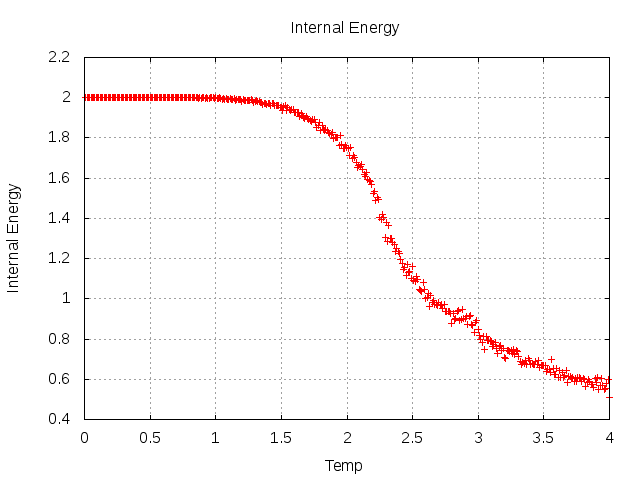
\includegraphics[width=0.75\textwidth]{EVsT.png}
%    %    \end{subfigure}
%\end{figure}
\subsection{Heat Capacity}
%\begin{figure}[H]
%        \centering
%        \caption{Heat Capacity vs Temperature \label{fig:CvsT}}
%    %    \begin{subfigure}[b]{\textwidth}
%                \centering
%                \includegraphics[width=0.75\textwidth]{CVsT.png}
%    %    \end{subfigure}
%\end{figure}
\subsection{Critical Exponents}
%\begin{figure}[H]
%        \centering
%        \caption{log(Magnetic Susceptibility) vs log(Temperature) \label{fig:logchivslogT}}
%    %    \begin{subfigure}[b]{\textwidth}
%                \centering
%                \includegraphics[width=0.75\textwidth]{logchiVslogT.png}
%    %    \end{subfigure}
%\end{figure}
%\begin{figure}[H]
%        \centering
%        \caption{log(Heat Capacity) vs log(Temperature) \label{fig:logCvslogT}}
%    %    \begin{subfigure}[b]{\textwidth}
%                \centering
%                \includegraphics[width=0.75\textwidth]{logCVslogT.png}
%    %    \end{subfigure}
%\end{figure}
\newpage
\thispagestyle{empty}
\mbox{}

\newpage
\section{References}
\begin{thebibliography}{99}
\bibitem{JM} Thijssen, J. M. \textit{Computational Physics}. Ch. 8. Cambridge University Press. 1999. Print.
\end{thebibliography}

\end{document}
